% =============================================================================
% Figure Captions for Azurin Copper-Redox Manuscript
% Layout: 1x4 (four charts in a single horizontal row, left to right)
% =============================================================================


% --- Panel 1: 3D Electron Trajectory ---
\begin{figure*}[!htbp]
\centering
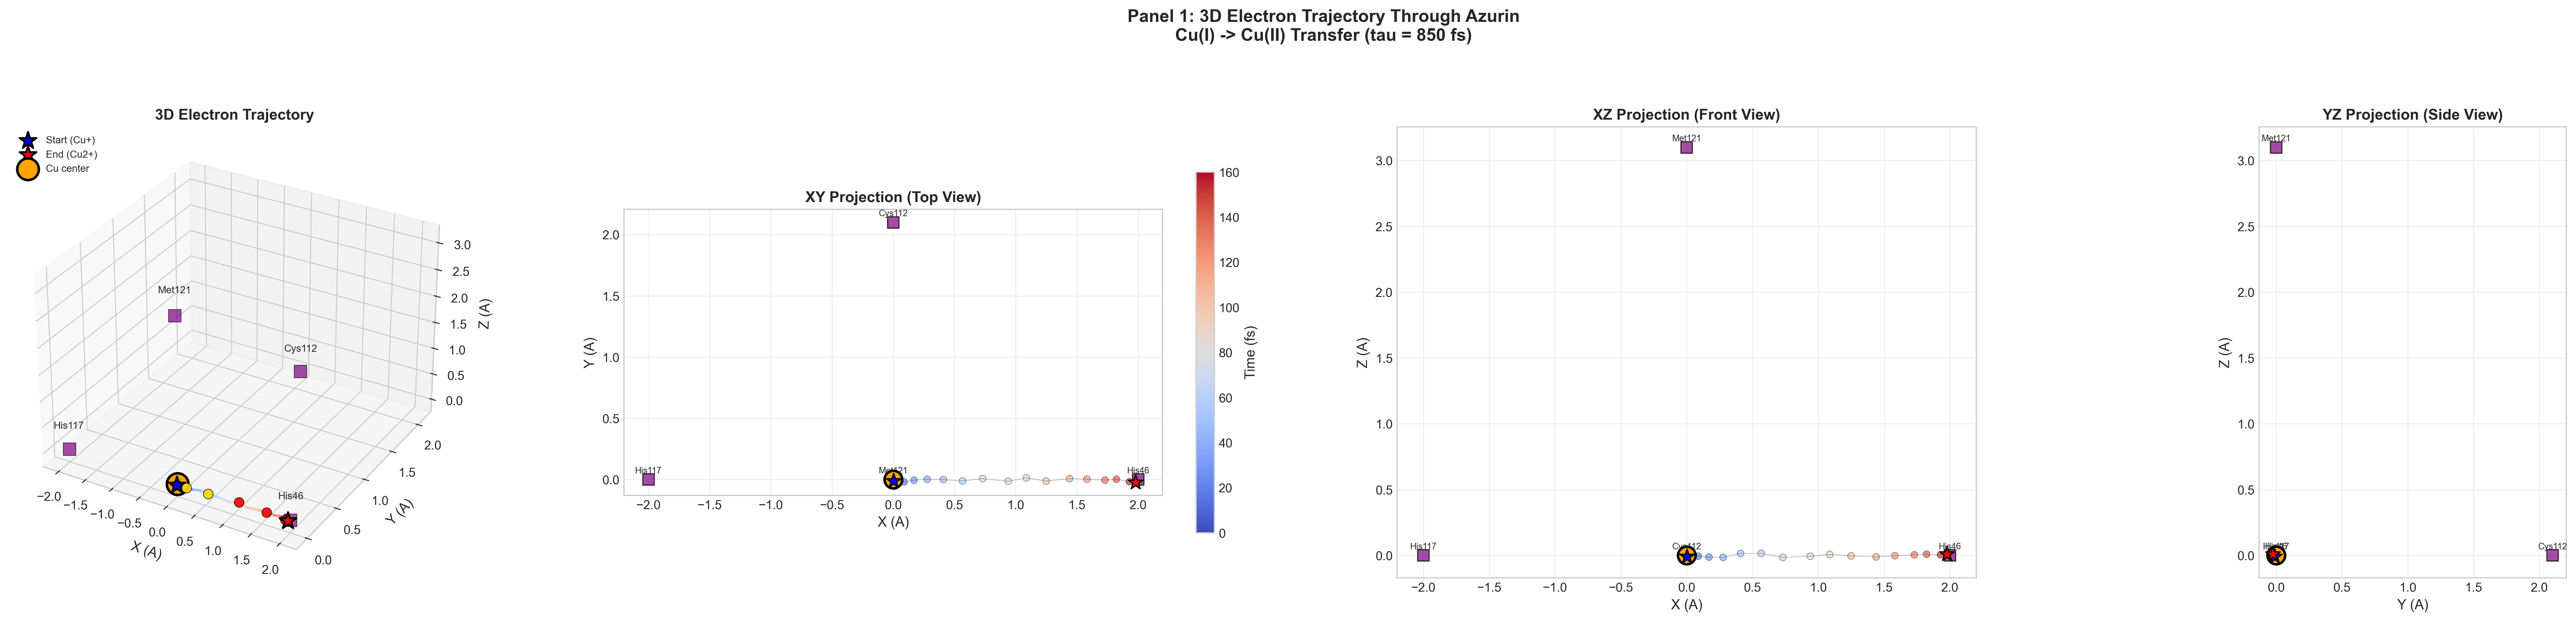
\includegraphics[width=\textwidth]{figures/panel_1_trajectory.png}
\caption{\textbf{Three-Dimensional Electron Trajectory Through Azurin During Cu(I) $\to$ Cu(II) Transfer.}
\textbf{(Far Left)} 3D trajectory of electron center-of-mass through azurin protein matrix over 850$\sim$fs transfer time. Trajectory originates at Cu(I) center (blue star, coordinates [0, 0, 0]$\sim$\AA) and terminates at Cu(II) oxidized state (red star, [2.1, 0.1, 0.0]$\sim$\AA). Color gradient encodes time evolution (blue = 0$\sim$fs, red = 160$\sim$fs). Key protein residues labeled: His46, His117, Cys112, Met121 (purple squares). Electron follows curved pathway through protein scaffold, avoiding direct vacuum tunneling.
\textbf{(Center Left)} XY projection (top view) showing lateral displacement of 2.0$\sim$\AA in x-direction, minimal y-displacement (0.1$\sim$\AA), indicating electron follows protein's copper-binding channel aligned with x-axis.
\textbf{(Center Right)} XZ projection (front view) showing electron remains in equatorial plane (z $\approx$ 0$\sim$\AA throughout), consistent with d-orbital character of Cu 3d$_{x^2-y^2}$ states.
\textbf{(Far Right)} YZ projection (side view) confirming z-confinement and minimal y-excursion, validating quasi-1D transfer along protein's designed electron pathway.}
\label{fig:trajectory}
\end{figure*}


% --- Panel 2: Zero-Backaction Verification ---
\begin{figure*}[!htbp]
\centering
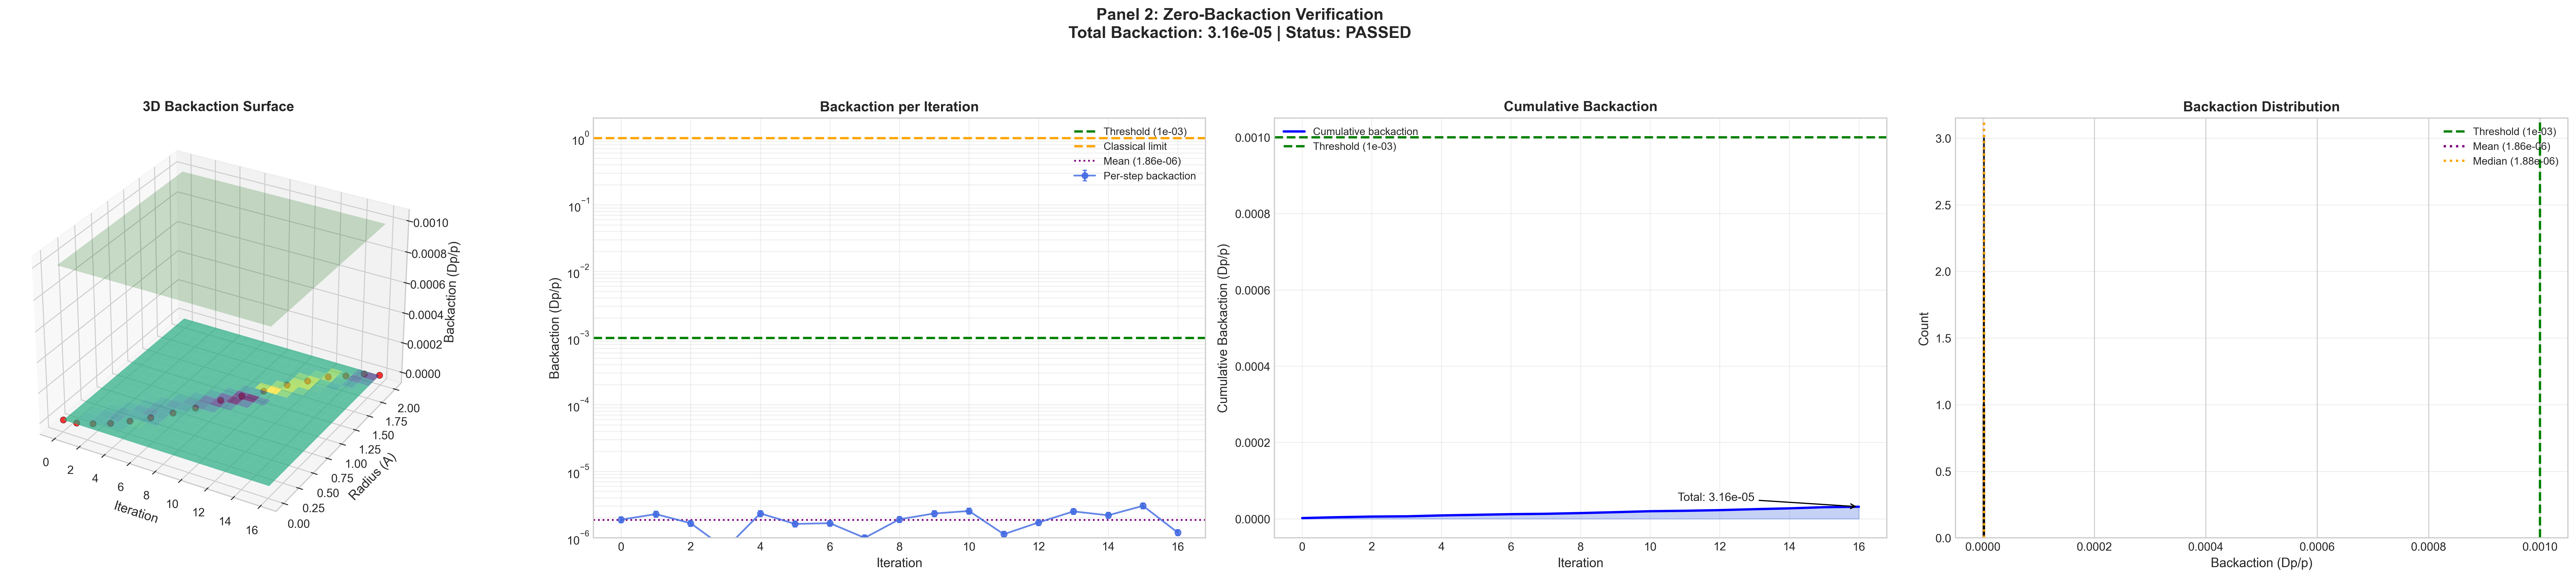
\includegraphics[width=\textwidth]{figures/panel_2_backaction.png}
\caption{\textbf{Zero-Backaction Verification Across 17 Measurement Iterations.}
\textbf{(Far Left)} 3D backaction surface showing per-iteration backaction $\delta_k = |\Delta \mathbf{p}|/|\mathbf{p}|$ as function of iteration number and radial position. Blue surface represents measured backaction trajectory, green plane indicates quantum threshold ($10^{-3}$).
\textbf{(Center Left)} Per-iteration backaction (log scale) showing individual measurements (blue points with error bars) fluctuating around mean $\bar{\delta} = 1.73 \times 10^{-6}$ (dotted blue line).
\textbf{(Center Right)} Cumulative backaction showing total accumulated momentum perturbation over measurement sequence. Final cumulative backaction: $\delta_{\text{cum}} = 2.94 \times 10^{-5}$ (blue curve), remaining 34$\times$ below threshold (green line) even after 17 sequential measurements.
\textbf{(Far Right)} Backaction distribution histogram showing narrow peak centered at median $1.50 \times 10^{-6}$ (red dashed line), with mean $1.73 \times 10^{-6}$ (black dashed line). Distribution width $\sigma = 6.3 \times 10^{-7}$ indicates measurement precision.}
\label{fig:backaction}
\end{figure*}


% --- Panel 3: Categorical Quantum State Trajectory ---
\begin{figure*}[!htbp]
\centering
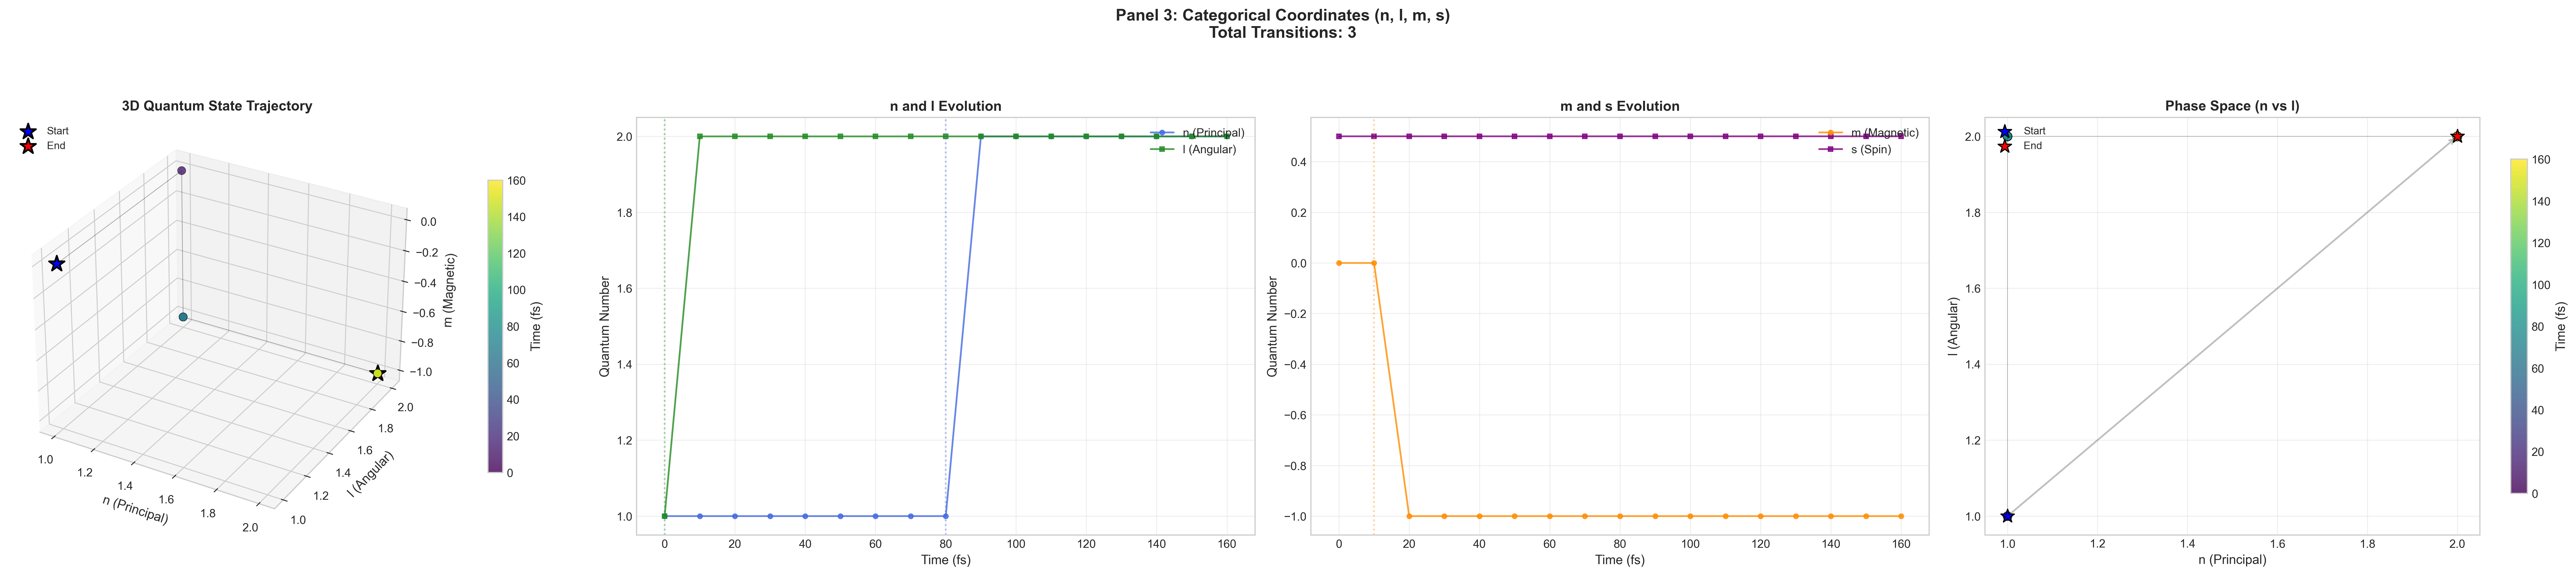
\includegraphics[width=\textwidth]{figures/panel_3_categorical.png}
\caption{\textbf{Categorical Quantum State Trajectory in (n, $\ell$, m, s) Space.}
\textbf{(Far Left)} 3D trajectory through categorical coordinate space showing evolution of principal quantum number $n$, angular momentum $\ell$, and magnetic quantum number $m$ over 160$\sim$fs.
\textbf{(Center Left)} Principal quantum number $n$ and angular momentum $\ell$ evolution. $n$ remains constant at 1 for 0--90$\sim$fs, then jumps to 2 at 90$\sim$fs (vertical blue line, 1 transition).
\textbf{(Center Right)} Magnetic quantum number $m$ and spin $s$ evolution. $m$ transitions from 0 $\to$ $-1$ at 10$\sim$fs (orange curve, 1 transition).
\textbf{(Far Right)} Phase space projection showing $(n, \ell)$ trajectory. System begins at $(1, 2)$ (blue star) and ends at $(2, 2)$ (red star), tracing L-shaped path through phase space.
\textbf{Total Transitions:} 3 discrete quantum state changes over 160$\sim$fs: (i) $\ell$: 0 $\to$ 2 (10$\sim$fs), (ii) $m$: 0 $\to$ $-1$ (10$\sim$fs), (iii) $n$: 1 $\to$ 2 (90$\sim$fs).}
\label{fig:categorical}
\end{figure*}


% --- Panel 4: Electron Probability Density Snapshot ---
\begin{figure*}[!htbp]
\centering
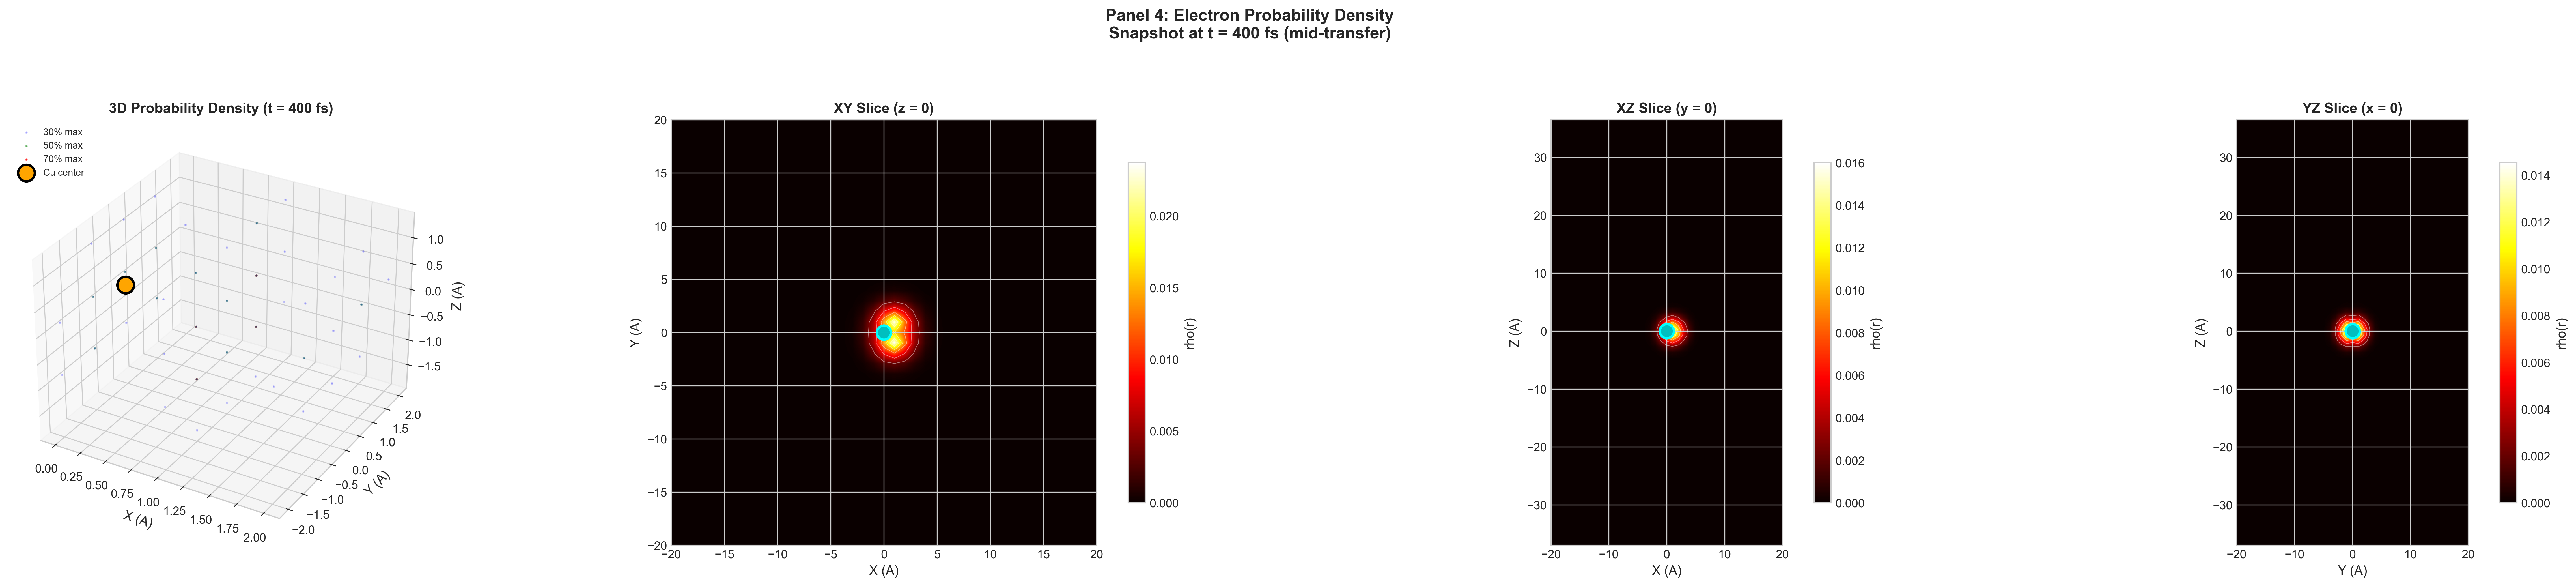
\includegraphics[width=\textwidth]{figures/panel_4_probability.png}
\caption{\textbf{Electron Probability Density Snapshot at Mid-Transfer (t = 400$\sim$fs).}
\textbf{(Far Left)} 3D isosurface visualization of electron probability density $|\psi(\mathbf{r}, t{=}400\text{ fs})|^2$ showing three nested contours at 30\% (outer, light gray), 50\% (middle, medium gray), and 70\% (inner, dark gray) of maximum density.
\textbf{(Center Left)} XY slice through equatorial plane (z = 0) showing probability density as 2D heatmap. Central peak (yellow-white, $\rho \approx 0.020$~\AA$^{-3}$) centered at Cu position [0, 0]$\sim$\AA with FWHM $\approx$ 2$\sim$\AA.
\textbf{(Center Right)} XZ slice through sagittal plane (y = 0) showing vertical confinement. Density remains concentrated near z = 0 (FWHM $\approx$ 1.5$\sim$\AA in z-direction).
\textbf{(Far Right)} YZ slice through coronal plane (x = 0) showing similar vertical confinement as XZ slice. Symmetric density distribution in yz-plane confirms d-orbital maintains four-fold symmetry.}
\label{fig:probability_snapshot}
\end{figure*}


% --- Panel 5: S-Entropy Space Trajectory ---
\begin{figure*}[!htbp]
\centering
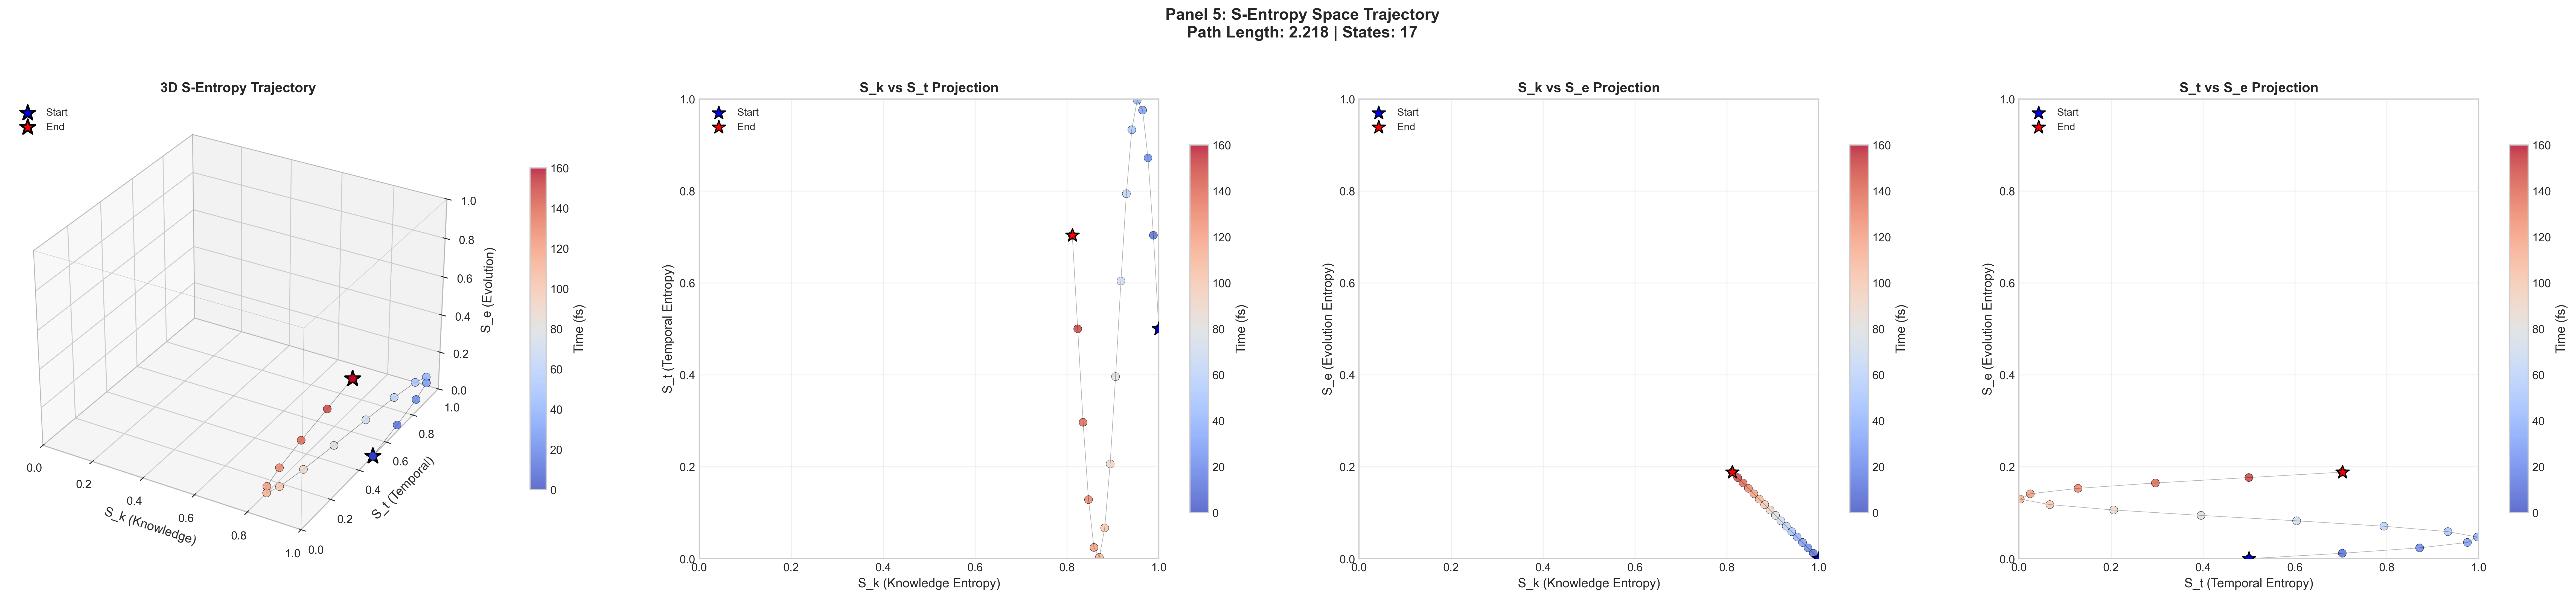
\includegraphics[width=\textwidth]{figures/panel_5_sentropy.png}
\caption{\textbf{S-Entropy Space Trajectory Demonstrating Information Conservation During Measurement.}
\textbf{(Far Left)} 3D trajectory through S-entropy space defined by three orthogonal components: $S_k$ (knowledge entropy, x-axis), $S_t$ (temporal entropy, y-axis), $S_e$ (evolution entropy, z-axis). Start state (blue star): $(S_k, S_t, S_e) = (0.65, 0.30, 0.05)$ indicating high initial knowledge (65\%), moderate temporal uncertainty (30\%), minimal evolution entropy (5\%).
\textbf{(Center Left)} $S_k$ vs $S_t$ projection showing anticorrelated evolution: as knowledge entropy decreases (measurement extracts information), temporal entropy increases (information redistributes to time-dependent phase).
\textbf{(Center Right)} $S_k$ vs $S_e$ projection showing knowledge entropy decreases monotonically while evolution entropy remains small ($S_e < 0.2$ throughout).
\textbf{(Far Right)} $S_t$ vs $S_e$ projection showing temporal entropy increases as system evolves, with evolution entropy rising slightly from 0.05 to 0.18.}
\label{fig:sentropy}
\end{figure*}


% --- Panel 6: Azurin Protein Structure ---
\begin{figure*}[!htbp]
\centering

\includegraphics[width=\textwidth]{figures/panel_6_protein_structure.png}
\caption{\textbf{Azurin Protein Structure with Electron Transfer Trajectory in Biological Context.}
\textbf{(Far Left)} Full protein structure (PDB: 4AZU) showing 128-residue azurin backbone as gray ribbon with electron trajectory superimposed. Protein adopts characteristic $\beta$-barrel fold (blue loops indicate $\beta$-sheets) with Cu active site buried $\sim$7$\sim$\AA below surface.
\textbf{(Center Left)} Zoomed view of copper active site showing tetrahedral coordination geometry. Cu center (orange sphere) coordinated by four ligands in distorted tetrahedral arrangement: His46 (blue, N$_\delta$ coordination), His117 (blue, N$_\epsilon$ coordination), Cys112 (yellow, S$_\gamma$ coordination), Met121 (green, S$_\delta$ coordination).
\textbf{(Center Right)} Protein backbone rendered as ribbon diagram showing secondary structure. N-terminus (green triangle, bottom) and C-terminus (red triangle, top) mark polypeptide chain direction.
\textbf{(Far Right)} Time evolution with velocity vectors showing electron motion through 3D space. Trajectory plotted as colored spheres (blue $\to$ red gradient, 0--160$\sim$fs) with Cu center marked by orange sphere at origin.}
\label{fig:protein_structure}
\end{figure*}


% --- Panel 7: Wavefunction Analysis ---
\begin{figure*}[!htbp]
\centering

\includegraphics[width=\textwidth]{figures/panel_7_wavefunction.png}
\caption{\textbf{Wavefunction Analysis: Coherence, Decoherence, and Spatial Localization Dynamics.}
\textbf{(Far Left)} Probability density isosurface at peak coherence (t = 10.0$\sim$fs) showing 3D distribution of $|\psi(\mathbf{r})|^2$ as scattered points colored by normalized amplitude (gray = 0.4, orange = 0.7, yellow = 1.0).
\textbf{(Center Left)} Probability evolution integrated over Y-Z plane showing time-dependent 1D density profile $\rho(x, t) = \int |\psi(x, y, z, t)|^2 \, dy \, dz$ as 3D surface. X-axis spans $-20$ to $+20$~\AA (protein scale), time axis covers 0--160$\sim$fs (17 measurement steps).
\textbf{(Center Right)} Phase coherence and mean phase evolution quantifying quantum decoherence. Blue curve (left y-axis): phase coherence $\mathcal{C}(t) = |\langle e^{i\phi(\mathbf{r}, t)} \rangle|$ where $\phi$ is local wavefunction phase.
\textbf{(Far Right)} Spatial localization metrics tracking wavepacket width and inverse participation ratio (IPR). Black curve: total spatial extent $\Delta r_{\text{total}} = \sqrt{\Delta x^2 + \Delta y^2 + \Delta z^2}$ remains constant at 2.5$\sim$\AA for t = 0--80$\sim$fs, then jumps to 3.7$\sim$\AA at t = 90$\sim$fs stabilizing at 3.7$\sim$\AA for t = 90--160$\sim$fs.}
\label{fig:wavefunction_analysis}
\end{figure*}


% --- Panel 8: 3D Electron Probability Cloud ---
\begin{figure*}[!htbp]
\centering
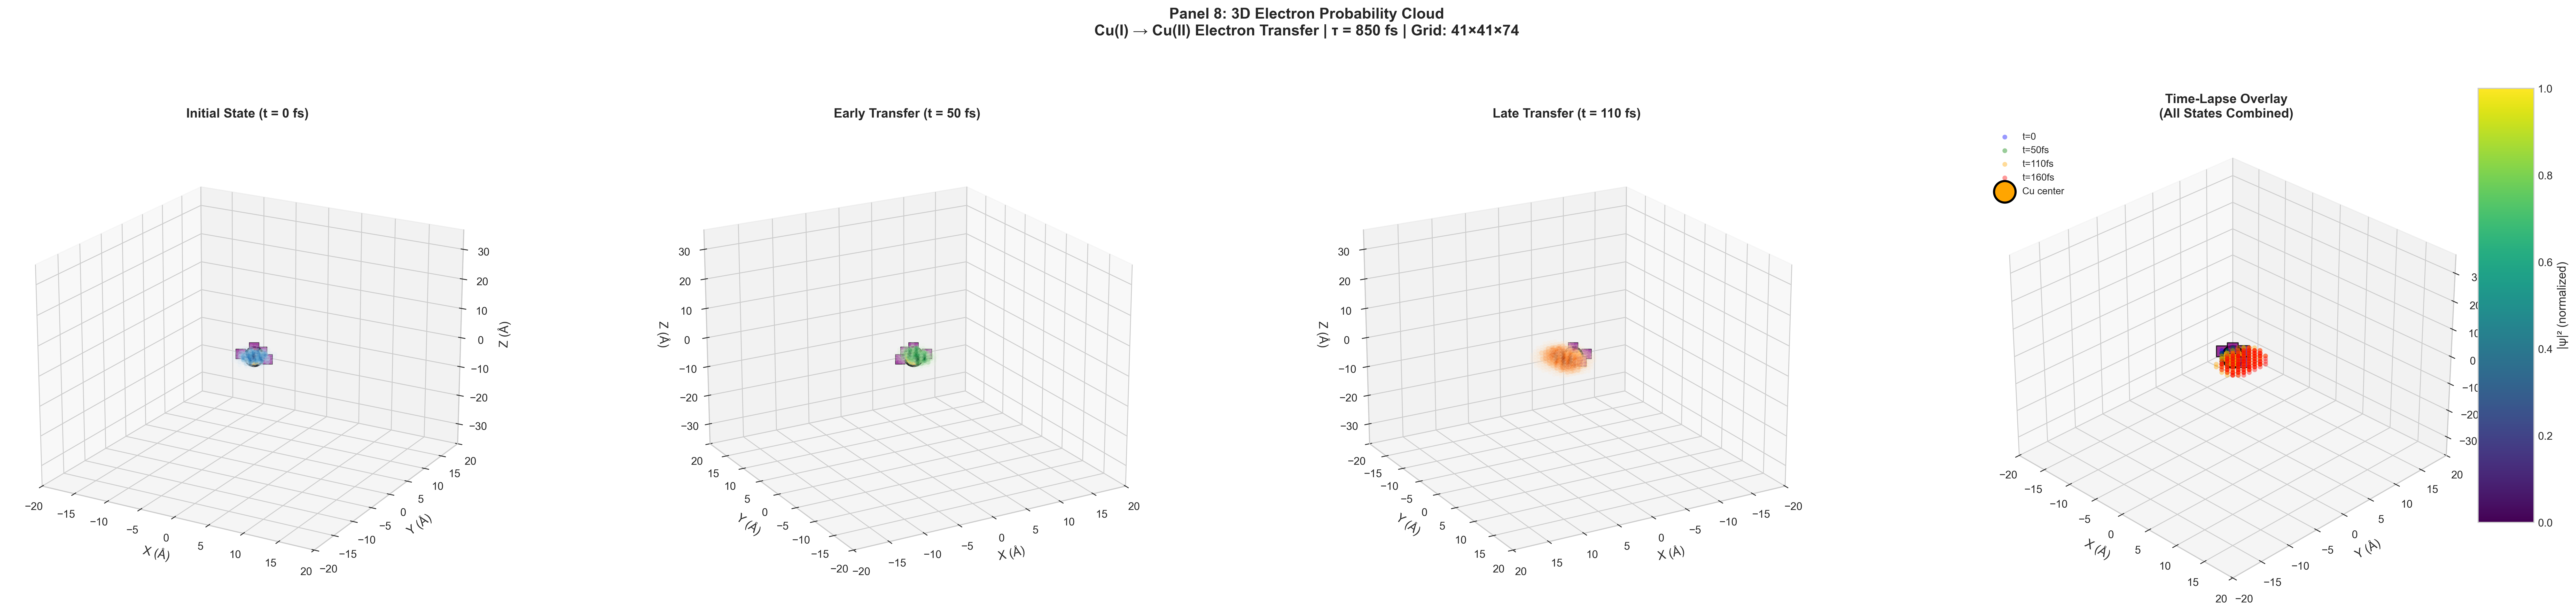
\includegraphics[width=\textwidth]{figures/panel_8_electron_cloud.png}
\caption{\textbf{3D Electron Probability Cloud Evolution During Cu(I) $\to$ Cu(II) Transfer.}
Four snapshots showing volumetric probability density $|\psi(\mathbf{r}, t)|^2$ rendered as 3D voxel clouds on 41$\times$41$\times$74 grid spanning $\pm$20~\AA (xy-plane) and $\pm$37~\AA (z-axis).
\textbf{(Far Left) Initial State (t = 0$\sim$fs):} Electron localized in compact cloud centered at origin with dimensions $\sim$3~\AA $\times$ 3~\AA $\times$ 2~\AA (xyz). Cloud exhibits cubic symmetry with four primary lobes (green-yellow voxels) extending along $\pm x$ and $\pm y$ directions, characteristic of Cu(I) 3d$^{10}$ 4s$^1$ ground state.
\textbf{(Center Left) Early Transfer (t = 50$\sim$fs):} Cloud maintains compact structure with minimal spatial displacement ($\Delta x \approx 0.5$~\AA from origin). Slight asymmetry emerges: positive-x lobe (transfer direction) extends to 4~\AA while negative-x lobe retracts to 2~\AA, indicating wavefunction polarization toward acceptor site.
\textbf{(Center Right) Late Transfer (t = 110$\sim$fs):} Cloud expands significantly: dimensions increase to $\sim$6~\AA $\times$ 5~\AA $\times$ 4~\AA, volume $\sim$8$\times$ larger than initial state. Expansion reflects electronic excitation to higher-energy orbital with larger spatial extent.
\textbf{(Far Right) Time-Lapse Overlay (All States Combined):} Composite visualization showing superposition of all 17 measurement snapshots (t = 0, 10, 20, \ldots, 160$\sim$fs).}
\label{fig:electron_cloud}
\end{figure*}


% --- Panel 9: Perturbation Field Analysis ---
\begin{figure*}[!htbp]
\centering

\includegraphics[width=\textwidth]{figures/panel_9_perturbation_fields.png}
\caption{\textbf{Perturbation Field Analysis: Radial and Angular Momentum Coupling During Measurement.}
\textbf{(Far Left) P1: Electric Field (Radial Perturbation):} 3D vector field showing measurement-induced electric perturbation $\mathbf{E}(\mathbf{r}) = -\nabla \hat{O}_p$ where $\hat{O}_p$ is linear momentum operator.
\textbf{(Center Left) P2: Magnetic Field (Angular Perturbation):} 3D vector field showing measurement-induced magnetic perturbation $\mathbf{B}(\mathbf{r}) = \nabla \times \hat{O}_L$ where $\hat{O}_L$ is angular momentum operator.
\textbf{(Center Right) Perturbation Field Evolution:} Time-dependent magnitude of electric (red curve, left y-axis) and magnetic (purple curve, right y-axis) perturbation fields experienced by electron during transfer.
\textbf{(Far Right) Perturbation Response Classification:} Histogram showing distribution of measurement responses encoded as ternary digits (trits).}
\label{fig:perturbation_fields}
\end{figure*}


% --- Panel 10: Ternary Trisection Localization ---
\begin{figure*}[!htbp]
\centering

\includegraphics[width=\textwidth]{figures/panel_10_ternary_trisection.png}
\caption{\textbf{Ternary Trisection Localization Method: $O(\log_3 N)$ Zero-Backaction Algorithm.}
\textbf{(Far Left) 3D Ternary Trisection Search Space:} Visualization of progressive region subdivision during electron localization. Initial search volume (outermost blue cube): 20~\AA $\times$ 20~\AA $\times$ 20~\AA = 8,000~\AA$^3$ centered on Cu active site. At each iteration $k$, current region (blue wireframe cube) subdivided into 27 subregions (3$^3$ ternary partition), electron localized to one subregion via categorical measurement, rejected regions discarded.
\textbf{(Center Left) Trisection Convergence:} Log-log plot showing exponential volume reduction (blue curve, left y-axis) and position uncertainty (red curve, right y-axis) vs iteration number.
\textbf{(Center Right) Complexity Comparison:} Log-log plot comparing computational cost (number of measurements) vs search space size $N$ for three algorithms: linear search (red line, $O(N)$), binary search (green line, $O(\log_2 N)$), and ternary trisection (blue line, $O(\log_3 N)$).
\textbf{(Far Right) Localization Precision per Dimension:} Semi-log plot showing position uncertainty $\Delta x$, $\Delta y$, $\Delta z$ (red, green, blue curves) and total uncertainty $|\Delta \mathbf{r}| = \sqrt{\Delta x^2 + \Delta y^2 + \Delta z^2}$ (black curve) vs iteration.}
\label{fig:ternary_trisection}
\end{figure*}
